\section{Probleemi uurimine}

Ehitusfüüsika mõistes ehituskonstruktsioon kujutab endast erinevate füüsikaliste oma-dustega kihtidest 
koosnevat struktuuri, mis eraldab kaks erinevat keskkonda (näiteks: hoone sees olev õhk ja õues olev õhk).
Seejuures kõige olulisemad materjalide omadused on soojuserijuhtivus \begin{math}\lambda\end{math} [W/mK]
ja veeaurutakistus, mis võib olla väljendatud mitmel viisil (neid viise on palju, aga käesolevas töös keskendutakse 
ainult järgmistele, kuna need on kõige rohkem kasutatud nii raamatutes, kui ka materjalitootjate dokumentatsioonis):
\begin{math}\mu\end{math} - diffusioonitakistustegur (materjali omadus), Sd[m] - suhteline diffusioonitakistus 
(kindla paksusega toote omadus). 

\begin{figure}[ht]
    \centering
    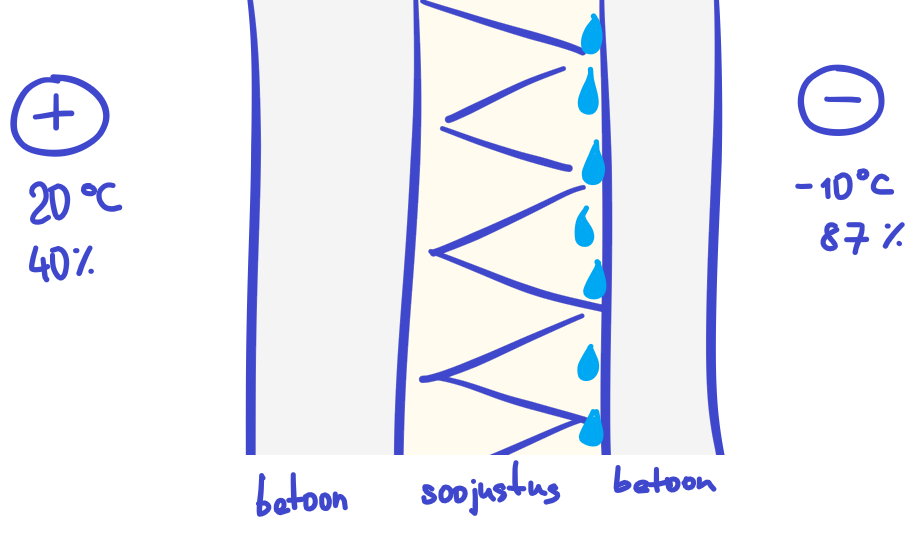
\includegraphics[width=.6\textwidth]{figures/problem_statement/07_layered_structure_sample.png}
    \caption[Mitmest kihist koosneva ehituskonstruktsiooni näide]{\textit{Kihilise konstruktsiooni näide}}
    \label{fig:construction_sample}
\end{figure}

Teatud tingimustel võib tekkida olukord, kui konstruktsiooni sees on mingis punktis suhteline niiskus
nii kõrge, et soodustab bioloogiliste kahjustuste või isegi kondensaadi tekkimist. Nimetatud olukord on ohtlik
nii ehituskonstruktsioonile, mis pikaajalise niiskuse mõjul lagunevad, kui ka inimese tervisele, sest konstruktsioonide
sees olev hallitus on õhku sattuvate bakterite allikaks. Seda, kuidas konstruktsioon töötab soojus- ja niiskuse leviku
seisukohalt nimetatakse konstruktsiooni niiskustehniliseks toimivuseks. Arvutust, mille eesmärgiks on hinnata 
kondenseerumise riski konstruktsioonis, nimetatakse konstruktsiooni niiskustehnilise toimivuse analüüsiks.

Tegemist on klassikalise ehitusfüüsika ülesandega, mille lehandemiseks peab ette võtma järgmiseid samme:
\begin{itemize}
    \item konstruktsiooni kihtide soojustakistuse ja konstruktsiooni summaarse soojustakistuse arvtus
    \item temperatuuri jaotuse määramine kihtides sõltuvalt sise- ja väliskeskkonna temperatuuridest ning 
    soojustakistuste väärtustest
    \item konstruktsiooni kihtide veeaurutakistuse ja konstruktsiooni summaarse veeaurutakistuse arvutus
    \item veeauru küllastusrõhu jaotuse määramine lähtuvalt temperatuuri jaotusest
    \item veeauru osarõhu jaotuse määramine kihides sõltuvalt sise- ja väliskeskkonna parameetritest ning 
    veeaurutakistuse väärtustest
    \item tulemuste esitamine graafiliselt diagrammil
    \item arvutuste kordamine erinevate sise- ja väliskeskkonna parameetrite kombinatsioonidega
\end{itemize}

Ülesande käsitsi lahendades, koostatakse tabelit, mille ridadesse pannakse kirja kihid ja veergudesse arvutatakse 
väärtused. Kuigi arvutused ise ei ole väga keerulised (tegemist on tavaliste füüsika valemitega), paraku käsitsi arvutamine 
võtab tohutult palju aega. Microsoft Excel võimaldab teatud määral protessi automatiseerida, kuid siiski mõned 
tegevused (näiteks uute kihtide lisamine, või kihtide järjekorra muutmine) jäävad suures osas käsitööks, mis võtab palju 
aega ja ka soodustab vea tegemist. Pildil \ref{fig:excel_table_sample} on toodud sellise tabeli näide.
\begin{figure}[ht]
    \centering
    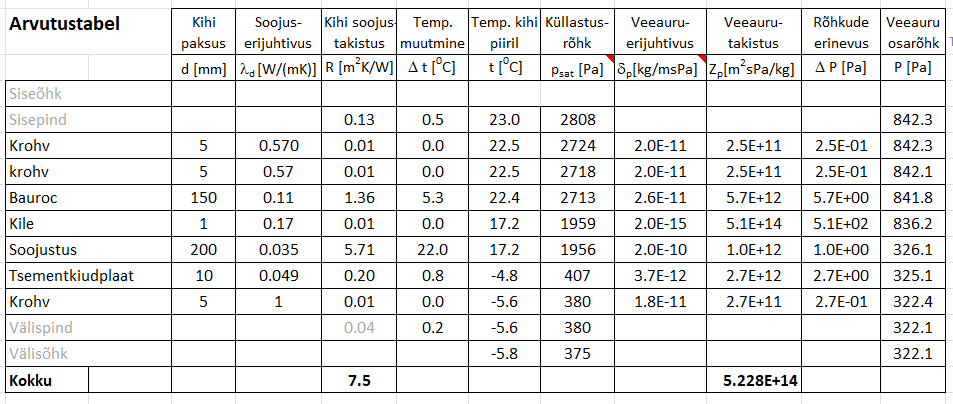
\includegraphics[width=.8\textwidth]{figures/problem_statement/04_calc_table.png}
    \caption[Näide niiskustehnilise analüüsi tulemuste esitamisest tabelis]{\textit{Arvutustabeli näide}}
    \label{fig:excel_table_sample}
\end{figure}

Analüüsi tulemused esitatakse graafiliselt diagrammi kujul, mille \begin{math}x\end{math} telg on 
punkti asukoht konstruktsioonis ning \begin{math}y\end{math} teljel on temperatuuri, veeauru küllastus- ja
osarõhu väärtused vastavas punktis -- näide on todud pildil  \ref{fig:excel_graph_sample}.

\begin{figure}[ht]
    \centering
    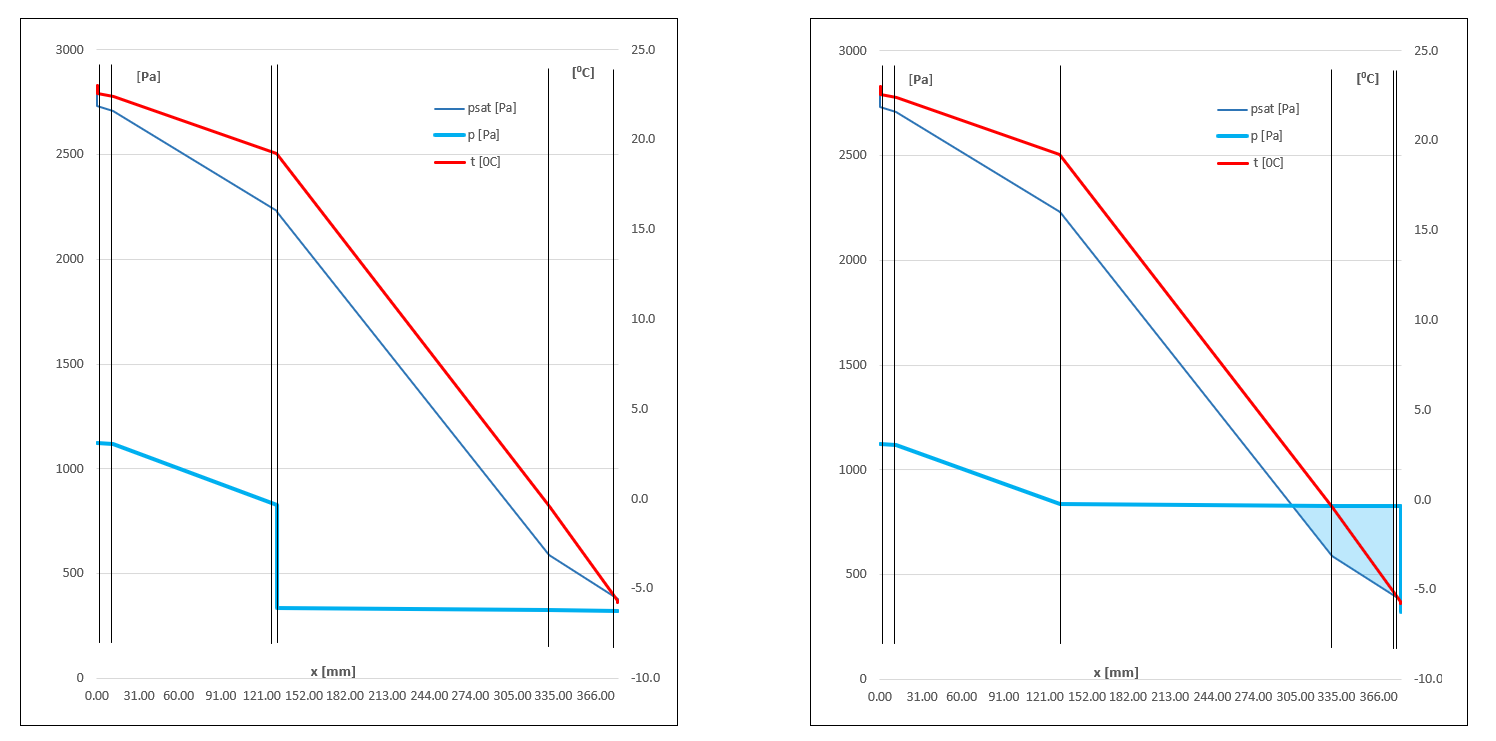
\includegraphics[width=.8\textwidth]{figures/problem_statement/05_excel_grafic_sample.png}
    \caption[Näide niiskustehnilise analüüsi tulemuste esitamisest graafikul]{\textit{Näide tulemuste esitamisest graafikul}}
    \label{fig:excel_graph_sample}
\end{figure}

Graafik annab väga head visuaalset ülevaadet konstruktsiooni kihtides toimuvale. Täpsemalt öeldes peab vaatama 
veeauru küllastus- ja osarõhkude jaotuste graafikuid. Veeauru osa- ja küllastusrõhu suhe on suhteline niiskus. 
Mida lähedam osarõhu graafiku joon küllastusrõhu graafiku joonele, seda kõrgem on suhteline niiskus. Punkt, milles
need jooned ristuvad on suhteline niiskus 100\%, mis tähendab kondensaadi tekkimist --  sellist punkti nimetatakse kastepunktiks.
Näide on toodud pildil \ref{fig:excel_graph_sample}: vasakul on niiskustehniline olukord hea, kuna aurutõke asub õiges kohas, ning paremal
paiknem konstruktsiooni külmemal pool veeaurupidav kiht, mistõttu läheb osarõhk kõrgeks ja ületab küllastusrõhu väärtust.

Kuigi probleem on üldjoontes lahendatav näiteks \textit{Microsoft Excel} vahenditega, paraku pole see kõige mugavam viis
mitmel põhjusel. Selline lähenemine vajab palju käsitööd kihtide lisamiseks või ümber paigutamiseks, mis on analüüsi lahutamata
osa -- proovitakse erinevaid materjale erinevates konstruktsiooni kohtades. Samuti materjalide andmeid on siiski vaja otsida 
ning hallata nende aktuaalsust ja usaldusväärsust -- aeganõudev töö, mida võiks elimineerida kasutades valmistoodet.


\section{Olemasolevad lahendused ja turu analüüs}
Üks populaarsematest analoogsetest lahendustest, mis on inseneridel kasutusel Euroopas, sealhulgas ka Eestis, on Saksa päritoluga tarkvara \textbf{Ubakus}. 
Tegemist on kommertstarkvaraga, mis töötab veebirkenduse kujul. Tarvara \textit{demo}-versioon on saadaval tasuta.
\begin{figure}[ht]
    \centering
    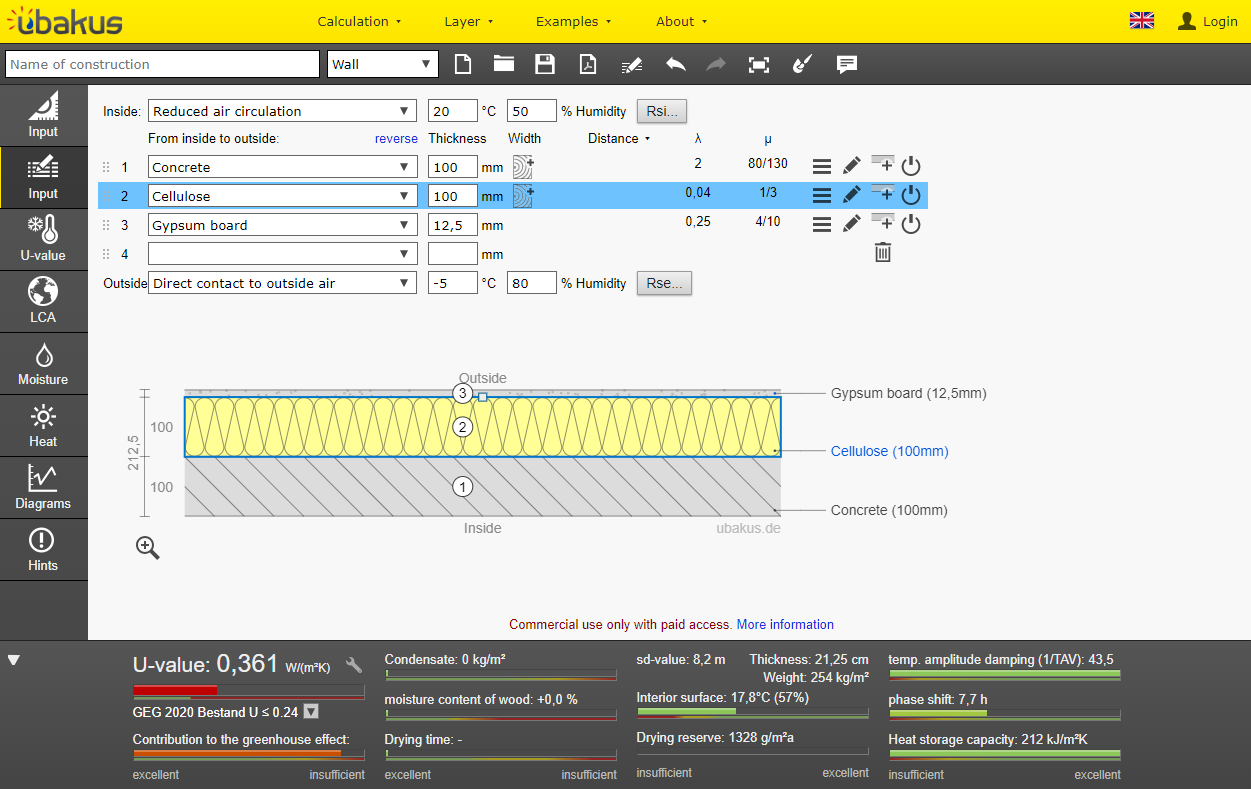
\includegraphics[width=.8\textwidth]{figures/problem_statement/01_ubakus.png}
    \caption[Ubakus tarkvara katutajaliides, ekraanitõmmis]{\textit{Ubakus: kasutajaliides, ekraanitõmmis.}}
    \label{fig:ubakus_sample}
\end{figure}

\textbf{Ubakus} võimaldab teostada konstruktsiooni niiskustehnilist analüüsi. Kasutajaliides võidaldab 
mudeldada mitmest kihist koosneva konstruktsiooni, valides igale kihile paksust ja materjali, millest 
kiht koosneb. Tugev eelis on see, et tarkvaraga saab analüüsida ka mittehomogeensete (mitemest erinevast 
materjalist, nt puitsõrestiksein) kihtidega konstruktsioone -- pilt \ref{fig:ubakus_sample}

Ehitusmaterjalide valik, mida on võimalik konstruktsiooni mudeldamisel kasutada, on piisavalt lai 
(aga tasuta versioonis piiratud). Tasulises versioonis on samuti võimalik ka oma materjalide 
lisamine ja kasutamine. Osa materjalidest on abstraktsed (näiteks: betoon, puit, mineraalvill), osa
on reaalsed turustatavad tooted (näiteks: Isover soojusisolatsioonide valik) -- pilt \ref{fig:ubakus_materials}. Võib puuduseks pidada
seda, et osa materjale (konkreetsed toted) on Saksamaal ja Kesk-Euroopas turustatavad materjalid, mistõttu selle 
tarkvara kasutades Eestis peab kas sisestama vajalikud kohalikud materjalid käsitsi, või arvestada Saksa analoogide
kasutusest tuleneva arvutuste ebatäpsusega.
\begin{figure}[ht]
    \centering
    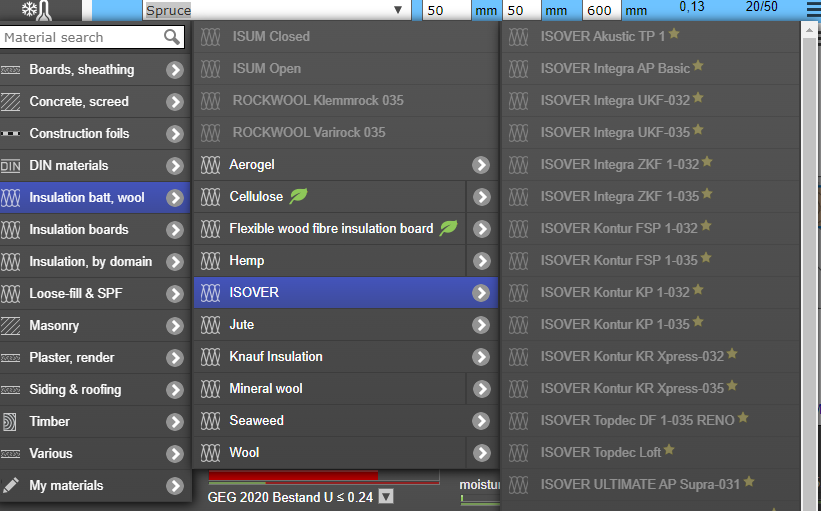
\includegraphics[width=.6\textwidth]{figures/problem_statement/03_ubakus_materials.png}
    \caption[Ubakus tarkvara materjalide valik, ekraanitõmmis]{\textit{Ubakus: ehitusmaterjalide valik baasis, ekraanitõmmis.}}
    \label{fig:ubakus_materials}
\end{figure}

Keskkonnatingimused valitakse manuaalselt sisestades õhutemperatuuri ja -niiskuse väärtused. Rakendus võimaldab arvutuste tulemust
vaadata erineval viisil, alates lihtsamast 3D visualiseeringust kuni värvilise temperatuurikaardini. Tarkavara saab osa aastase 
tellimusega, mille maksumus on alates 50 kuni 120 eurot sõltuvalt valitud paketist. Objektiivselt vaadates on tarkvara hea nii
funktsionaalsuse kui ka hinna seisukohalt. Lisaks sellele on ka kasutajaliides piisavalt mugav ja intuitiivselt arusaadav,
et seda saaks kasutada ka inimene, kellel puuduvad sügavad teadmised valdkonnast. Nagu varem oli mainitud, 
takvara on suunatud eelkõige Kesk-Euroopa ja Canada turgudele, Balti ja Skandinaavia riigidele lokaliseerimine puudub. Kokkuvõttes
antud lahendust võib kindlasti võtta arvesse toote funktsionaalsuse kavandamisel.

\textbf{Physibel Glasta} on üks analoogne lahendus veel, mis on samuti kommertstarkvara. Tegemist on samuti arvutile paigaldatava tarkvaraga, mille
kasutajaliides on veidi keerulisem ja ka disain on oluliselt konservatiivsem (pilt \ref{fig:glasta_sample}). 
\begin{figure}[ht]
    \centering
    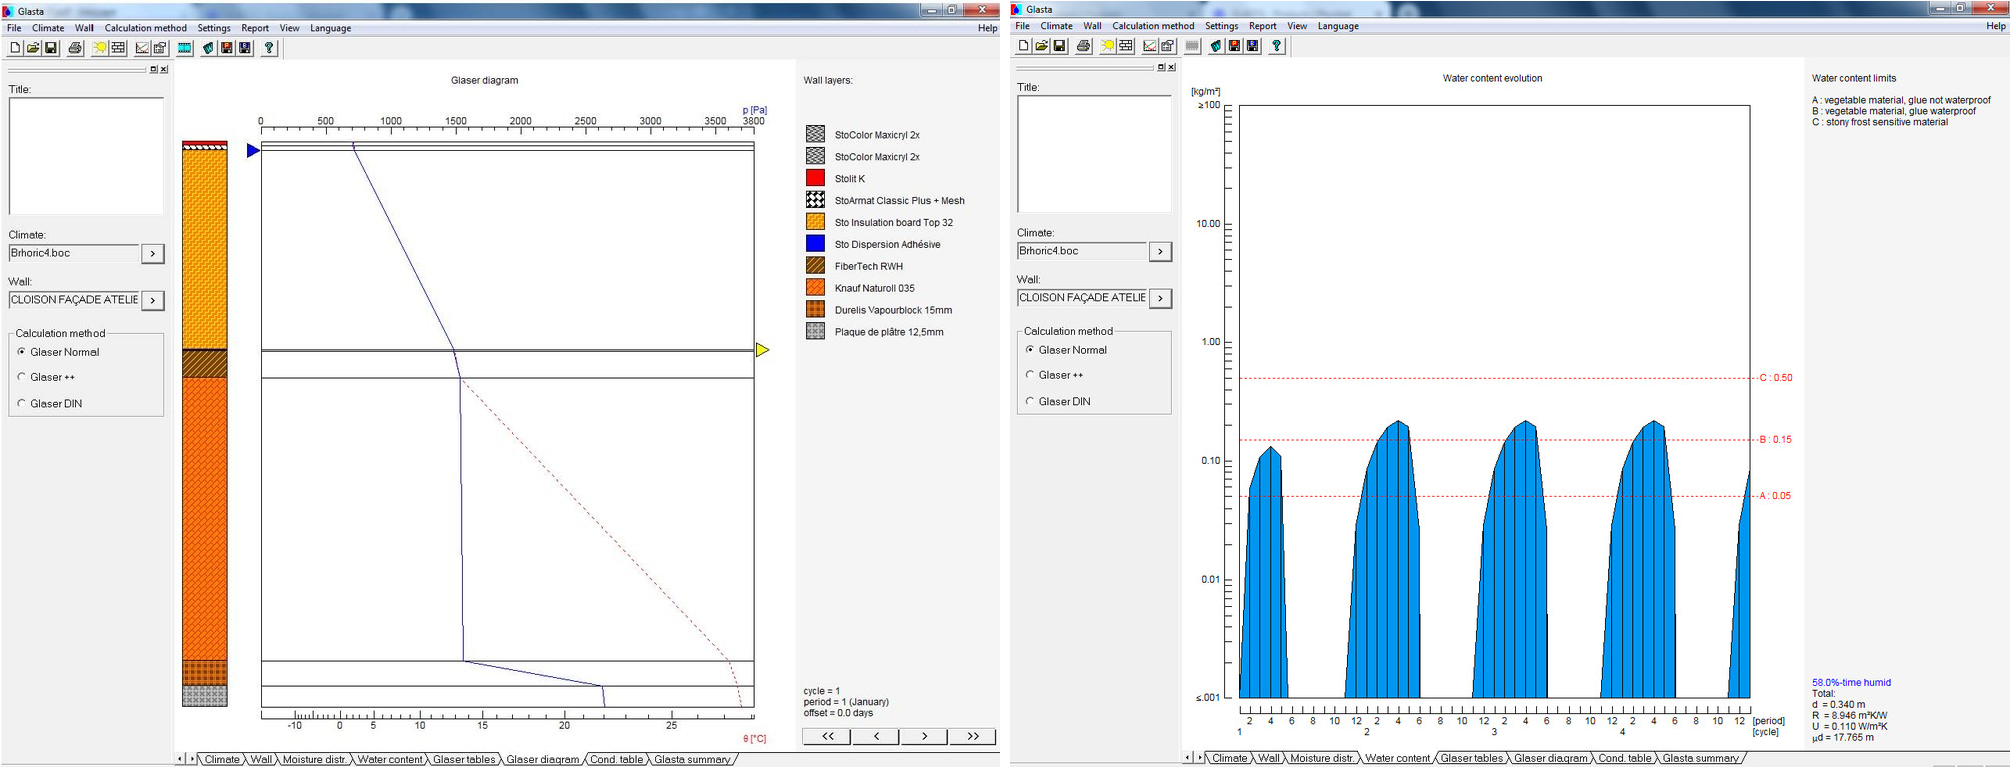
\includegraphics[width=.6\textwidth]{figures/problem_statement/09_glasta_sample.png}
    \caption[Physibel Glasta kasutajaliides, ekraanitõmmis]{\textit{Glasta: kasutajaliides, ekraanitõmmis.}}
    \label{fig:glasta_sample}
\end{figure}

Selle tarkvara funktsionaalsuse tugev eelis on võimalus teostada analüüsi aasta lõikes - väga tihti 
kondenseerumise probleem esineb vaid teatud perioodil (tavaliselt külmal hooajal),
ülejäänud ajal toimub kuivamine. See, et ühel või kahel talvisel kuul esineb konstruktsioonis kondenseerumise oht ei pruugi
olla probleemiks, kui ülejäänud ajal jõuab konstruktsioon täielikult kuivada. Antud asjaolu Glasta tarkvara analüüsib ning 
tulemust esitatakse ka graafikul (pilt \ref{fig:glasta_results}). Antud funktsionaalsus on äärmiselt oluline ja selle vajadusega peab toote 
planeerimisel arvestama. Tarkvara hind on suurusjärgus 500 eurot aastas, mis on päris kõrge, ning lisaks ka alla laadimise ja 
paigaldamise vajadus teeb antud lahendust ebamugavaks ja paljudel juhtudel ebaotstarbekaks.
\begin{figure}[ht]
    \centering
    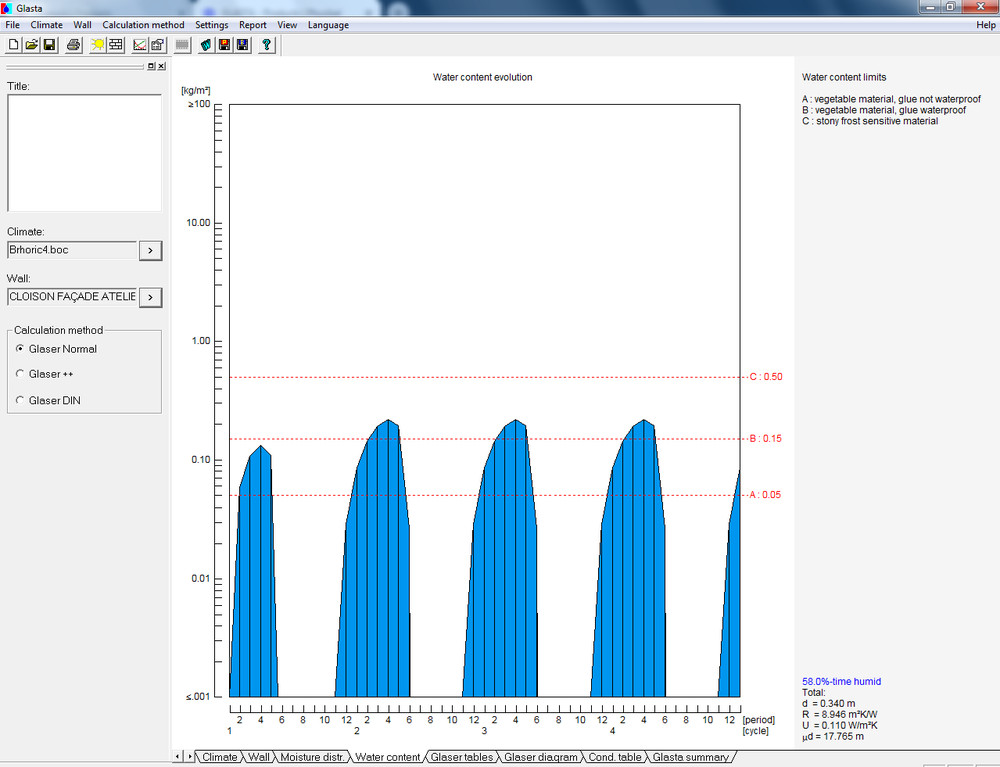
\includegraphics[width=.6\textwidth]{figures/problem_statement/10_glasta_results.png}
    \caption[Physibel Glasta tulemuste esitamine diagrammil, ekraanitõmmis]{\textit{Glasta: tulemuste esineamine diagrammil, ekraanitõmmis.}}
    \label{fig:glasta_results}
\end{figure}

Valdkonnas on olemas ka oma lipulaev -- \textbf{Delphin} on professionaalne tarkvara, mille hind on suurusjärgus 1000-1500 eurot aastas.
Eelisteks on väga lai funktsionaalsus ning ka täielik vabadus konstruktsiooni ja keskkonna mudeldamisel. Viimane on ühtlasi ka puuduseks,
sest kliimatingimuste mudeldamine eeldab ilmatingimuste (sealhulgas ka andmed päikesekiirgusest, sademetest) andmebaasi olemasolu.
Samuti vajab tarkvara ka kasutaja koolitust, mida tootja pakub ka pakub hinnaga 800 eurot. Eeltoodud asjaolud teevad antud tarkvara 
sobilikuks ja otstarbekaks vaid nendele, kellel ehitusfüüsika arvutused on põhitegevuseks.
